% id: 97-09
% book: 100발100중 3-2 기말 · 01 3-2 기말(원의 성질·통계·부록)
% section: 실전 모의고사 3회
% figure: crop:fig-97-09.png
% answer: ①
% answer_source: 답지(빠른정답)
% variant_level: 0 (원본 전사)
% 이 파일은 build.mjs 가 items.json 에서 만든다. 고칠 때는 items.json 을 고친다.
\smash{\raisebox{1.5mm}{\dmkichul{100발100중 3-2 기말 97쪽 09번}}}
\noindent\begin{minipage}[t]{0.58\linewidth}\vspace{0pt}\raggedright 그림에서 $\overleftrightarrow{\pt{PQ}}$는 두 원의 공통인 접선이고, 점~$\pt{T}$는 접점이다. $\angle\pt{TAB}=70^\circ$, $\angle\pt{PTA}=80^\circ$일 때, $\angle x-\angle y$의 크기는? \mbox{[3점]}\end{minipage}\hfill\begin{minipage}[t]{0.4\linewidth}\vspace{0pt}\centering 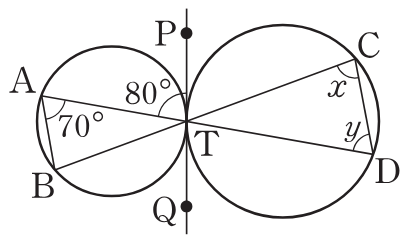
\includegraphics[width=98.1pt]{figures/fig-97-09.png}\end{minipage}\par
\begin{choices32}{$10^\circ$}{$15^\circ$}{$20^\circ$}{$30^\circ$}{$40^\circ$}\end{choices32}
